%=========================================================
% Block Diagram of SoC
%=========================================================
\section{Block Diagram of SoC}

Block diagram of mmRISC-1 Tiny SoC for FPGA is shown in Figure \ref{fig:BLOCKDIAGRAMJTAG} and Figure \ref{fig:BLOCKDIAGRAMCJTAG}. The former is the one with 4-wire JTAG debugger interface, and the the latter is the one with 2-wire cJTAG debugger interface.\\\\

The mmRISC-1 cpu core has 1 hart with RV32IMAC or RV32IMAFC ISA which is combined with JTAG Debugger. \\\\
Internal system bus is Multilayer Bus Matrix with AHB-Lite interface connecting CPU core, memories and all memory mapped peripheral devices. Instruction memory is a RAM with 1cyc read cycle time. Data memory is another RAM with 1cyc read cycle time and 1cyc write cycle time. \\\\
The SoC has simple SDRAM interface for 64MB (32MB x 16bit) SDRAM to expand work memory area.\\\\

UART is a simple asynchronous Tx/Rx device with configurable baud rate generator. 
I2C is a Inter Integrated Circuit for 2-wire serial communication interface. The SoC has 2-channel master I2C.
SPI is a Serial Peripheral Interface for synchronous communication interface. The SoC has 1-channel master SPI.
GPIO is general purpose Input Output with 32bits x 3ports. 
INT\_GEN and MTIME are peripherals described in mmRISC-1 chapter.\\\\

Reset is generated from external input or power-on-reset logic.\\
System clock frequency depends on configuration of CPU ISA according to result of timing analysis. As for the target FPGA, RV32IMAC without FPU configuration can operate in 20MHz wheres RV32IMAFC with FPU in 16.67MHz. The input clock frequency of the target board is 50MHz, so PLL makes appropriate clock frequency. \\\\

JTAG Debugger interface for OpenOCD is a handmade board using FTDI FT2232D chip which is almost compatible with commercial Olimex ARM-USB-OCD(H). Of course you can use the commercial product as JTAG interface.\\
As for the FPGA system with 4-wire JTAG debug interface as shown in Figure \ref{fig:BLOCKDIAGRAMJTAG}, the JTAG signals from USB to JTAG adapter with FTDI chip are connected to mmRISC-1 core directly.\\\\

On the other hand, as for the FPGA system with 2-wire cJTAG debug interface as shown in Figure \ref{fig:BLOCKDIAGRAMCJTAG}, the JTAG signals from USB to JTAG adapter with FTDI chip are inputted to the FPGA once, and "cJTAG Adapter" block converts them to 2-wire cJTAG signals which are connected to cJTAG\_2\_JTAG block through external loop back path, and at last the cJTAG\_2\_JTAG block converts cJTAG signals to JTAG signal which are connected to mmRISC-1 core.

\begin{figure}[H]
    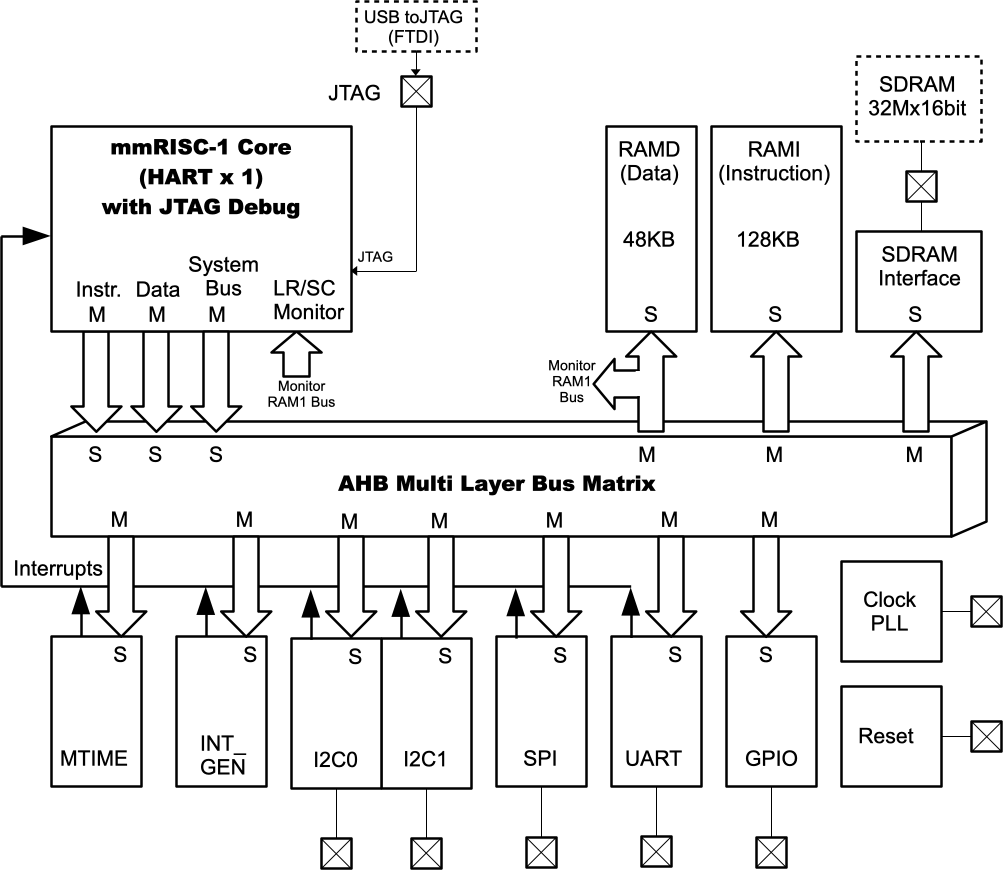
\includegraphics[width=0.8\columnwidth]{./Figure/BlockDiagramJTAG.png}
    \caption{Block Diagram of mmRISC-1 Tiny SoC for FPGA with 4-wire JTAG debug interface}
    \label{fig:BLOCKDIAGRAMJTAG}
\end{figure}

\begin{figure}[H]
    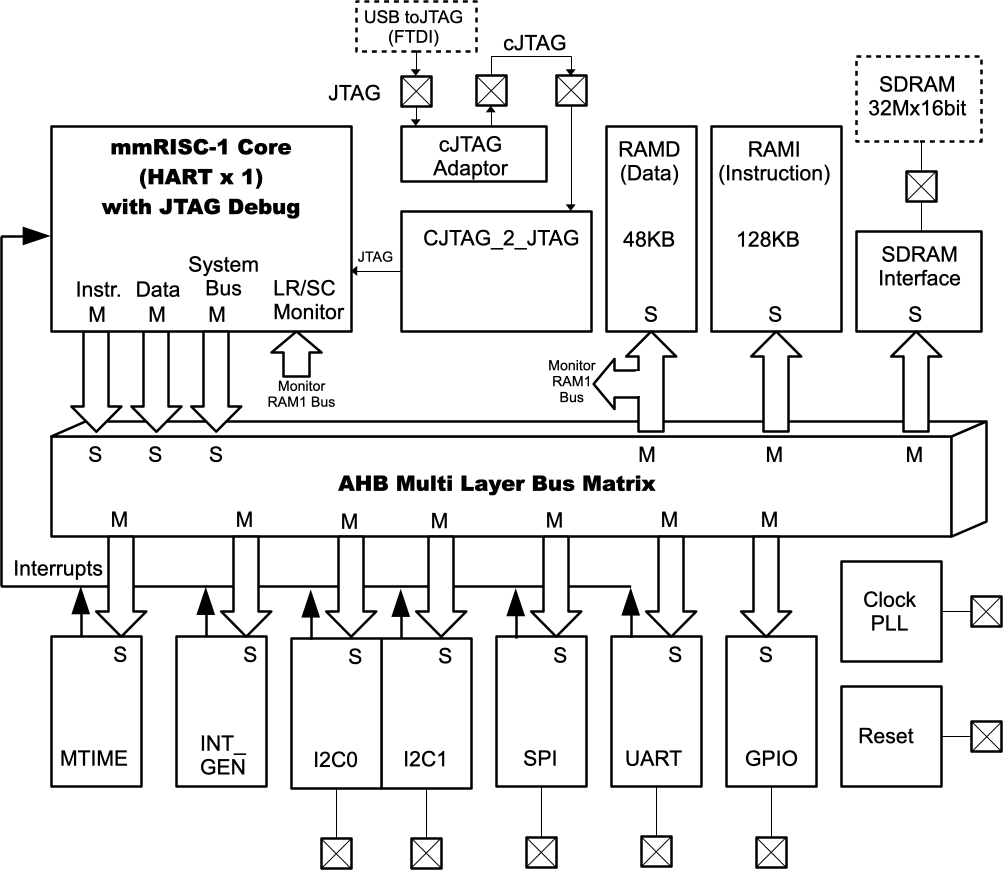
\includegraphics[width=0.8\columnwidth]{./Figure/BlockDiagramCJTAG.png}
    \caption{Block Diagram of mmRISC-1 Tiny SoC for FPGA with 2-wire cJTAG debug interface}
    \label{fig:BLOCKDIAGRAMCJTAG}
\end{figure}
